% This section is subsubsection crazy and all the whitespace ends up looking absurd.
% If needed, a similar block with the defaults can just be placed at the end of this section though.
% And if people prefer it like this, it can be moved to the preamble.
\titlespacing*{\subsubsection}
{0pt}{1ex}{0ex}

%%%%%%%%%% progress marker %%%%%%%%%%

%\section{Calibration Products Pipeline\\(\wbsCPP)}
\section{Calibration Products Production}
\label{sec:cpp}

This section details the input data and algorithms required to generate all data products necessary for the photometric calibration of the LSST survey. Details of the application of these products is covered in other sections of this document. The details of the input datasets are given in \secsymbol\ref{sec:CPP:inputs} and  \secsymbol\ref{sec:CPP:auxTelescope:inputs} , which define the source of these data, \ie which will be provided by the camera team and which will be measured on the mountain. Finally, sections \secsymbol\ref{sec:CPP:output} and \secsymbol\ref{sec:CPP:auxTelescope:outputs} list the various output data products from the Calibration Products Pipeline.

\subsection{Key Requirements}
\label{sec:CPP:keyRequirements}
The work performed in this WBS serves several complementary roles:

\begin{itemize}
 \item It will enable the production of calibration data products as required by the Level 2 Photometric Calibration Plan (\NewPCP{}) and other planning documents \cite{Lupton15}. This includes both characterization of the sensitivity of the LSST system (optics, filters and detector) and the transmissivity of, and emission from, the atmosphere;
 
 \item It will characterize detector anomalies in such a way that they can be corrected either by the instrument signature removal routines in the Single Frame Processing Pipeline (\wbsSFM) or, if appropriate, elsewhere in the system;
 
 \item It will provide updated values of the crosstalk matrix to the camera DAQ (for AP) and DM (for DRP) for correction of the raw data;
 
 \item It will allow for characterization of the optical ghosts and scattered light in the system.
\end{itemize}


%%%%%%%%%%%%%%%%%%%%%%%%%%%%%%%%%%%%%%%%%%%%%%%%%%
%%%%%%%%%%%%%%%%%%%%%%%%%%%%%%%%%%%%%%%%%%%%%%%%%%
%%%%%%%%%%%%%%%%%%%%%%%%%%%%%%%%%%%%%%%%%%%%%%%%%%

\subsection{Inputs}
\label{sec:CPP:inputs} 
The following section details the input datasets which will be available to the Calibration Products Pipeline which will be acquired by the operations team at some frequency TBD. Some of these will be acquired frequently, \eg flats, while some will be acquired much less frequently, \eg the gain and linearity values. It should be noted that these are the raw inputs, and as such, the algorithmic sections for items that are listed as camera team deliverables are shown as ``None'' as these will have been previously developed. However, many of these items are re-listed in the \hyperref[sec:CPP:output]{outputs section}, where the algorithms to recalculate/monitor these on the mountain are defined.


\subsubsection{Bias Frames}\label{sec:CPP:inputs:biases} 
A set of bias frames used for the production of the master bias frame, obtained by acquiring many zero second exposures with the shutter remaining closed, taken at the normal LSST cadence.
\alg None - these just need to be taken.


\subsubsection{Gain Values}\label{sec:CPP:inputs:gain} 
\cameraTeam
The gain values for all amplifiers in the camera, in \electron/ADU; note that these are required to high accuracy (0.1\%), as they are used in determination of the photometric flats.
\alg None.


\subsubsection{Linearity}\label{sec:CPP:inputs:linearityCurve} 
\cameraTeam
The linearity curve for each amplifier in the camera, as well as the level above which these non-linearity curves should be considered unreliable.
\alg None.


\subsubsection{Darks}\label{sec:CPP:inputs:dark}
Sets of long dark frames (\smalltilde 300s) with the actual exposure length optimized for the dark current in the delivered sensors, the delivered read-noise, and considering the trade-off against the integrated cosmic ray flux and radioisotope contamination.
\alg None - these just need to be taken.


\subsubsection{Crosstalk}\label{sec:CPP:inputs:crosstalk}
\cameraTeam
The crosstalk matrix for every pair of amplifiers in the camera. It is worth noting that this is expected to be a very sparse.
\alg None.


\subsubsection{Defect Map}\label{sec:CPP:inputs:defectList} 
\cameraTeam
A list of all bad (unusable) pixels in each CCD, as well as list of possibly suspect pixels, \ie ones which should be flagged as such during processing.
\alg None.


\subsubsection{Saturation levels}\label{sec:CPP:inputs:saturationLevel}
\cameraTeam
The lowest level (in electrons), for each amplifier, at which charge bleeds into the neighboring pixels. If necessary, they will also provide the level at which the serial register saturates (\ie if the serial saturates at a lower level than the parallels).
\alg None.


\subsubsection{Broadband Flats}\label{sec:CPP:inputs:broadFlat}
Sets of flats taken through the standard LSST filters. Flats will be taken at a number of flux levels to measure the \bfeffect coefficients and to check linearity, including sets of ``superflats'' - sets of high-flux flats with many repeats ($>50$, possibly $>100$). The superflats taken for \bfeffect characterization will not need to be taken regularly as this effect is not expected to evolve with time.
\alg None - these just need to be taken.


\subsubsection{Monochromatic Flats}\label{sec:CPP:inputs:monoFlat}
Sets of `monochromatic' (\c 1nm bandwidth and spacing) flat-field screen images taken with no filter/glass in the beam.
\alg None - these just need to be taken.


\subsubsection{CBP Data}\label{sec:CPP:inputs:CBP}
Sets of images taken with the Collimated Beam Projector (CBP). The proposed resolutions and steps in these datasets are preliminary. All CBP data will be processed using the standard LSST ISR, except without the application of flat-fielding. Standard LSST aperture photometry will then be used to measure the number of counts associated with each CBP spot.
\alg Scripting the CBP/8.4m to take each of these datasets in concert. The scripting/control requirements for the CBP are dealt with separately in \secsymbol\ref{sec:CPP:CBP_control}.


\paragraph{CBP dataset 1}\label{sec:CPP:inputs:CBP:mono}
Sets of CBP images scanned in wavelength at 1nm resolution\footnote{1nm `resolution' here denotes the bandwith of the light source, and can be this width, or any amount lower. It should, however, be noted that the accuracy on the wavelength calibration of the light source needs to be at the 0.1nm level.} every 1nm for a fixed set of spot positions on the camera, and for fixed footprint on M1. No filter should be in the beam.
%Add a reference to the DESC people showing that this is necessary for SN cosmology in LSST.?

	
\paragraph{CBP dataset 2}\label{sec:CPP:inputs:CBP:spot}
Sets of CBP images scanned in wavelength at 20nm bandwidth every 100nm, while rotating the CBP about a pupil to move the spot pattern around the camera for a fixed footprint on M1. No filter should be in the beam.

	
\paragraph{CBP dataset 3}\label{sec:CPP:inputs:CBP:M1}
Sets of CBP images scanned in wavelength at 20nm resolution every 100nm for a fixed set of spot positions on the camera, and for a number of footprints on M1; the minimum number of footprints is \c 6 for a 30cm CBP, but in reality the use of more pointings will be explored to test the assumption of azimuthal symmetry. No filter should be in the beam.


\paragraph{CBP dataset 4}\label{sec:CPP:inputs:CBP:filter}
Sets of CBP images scanned in wavelength at 1nm resolution every 1nm for a fixed set of spot positions on the camera, and for a fixed footprint on M1. Repeated for every filter. \Nb the wavelength range for each scan need only cover the range for which the filter transmits appreciable light.


\paragraph{CBP dataset 5}\label{sec:CPP:inputs:CBP:leak}
Sets of CBP images scanned in wavelength at 20nm resolution every 20nm for a fixed set of spot positions on the camera, and for fixed footprint on M1. Repeated for every filter.


\paragraph {CBP Crosstalk Measurement}\label{sec:CPP:inputs:CBP:crosstalk}
Sets of CBP images taken with a suitably-designed sparse mask to allow identification and measurement of all ghost images arising from electronic crosstalk. The simplest sparse mask would have only a single spot, used to illuminate each amplifier in the camera in turn (but less sparse solutions are likely also possible). The wavelengths used are unimportant, and there are no constraints on beam footprints on M1 or filter choice. This will be particularly necessary should LSST be operated in a slow-readout mode, for example for use with 30s integrations, as crosstalk coefficients would change considerably.


\subsubsection{Filter Transmission}\label{sec:CPP:inputs:filterTransmission}
The transmission curves (transmission as a function of wavelength) for each filter, as a function of filter position. This is to be delivered by the filter vendors rather than the camera team, but is input data which will not be measured by DM. The required resolution is 1nm or better, in keeping with the resolution of the monochromatic flats.
\alg None.
\begin{note}
	We need to check what the proposed wavelength resolution and accuracy the vendors are proposing to use for this is. I spoke to Steve Ritz at the AHM and he seemed very positive about the vendor's proposal for this, but we should check what the plan is.
\end{note}


\subsubsection{Atmospheric Characterization}\label{sec:CPP:inputs:atmosphericData}
These are the external measurements of atmospheric parameters, \eg the barometric pressure, ozone and temperature, provided by measurement systems both on and off site.
\alg Interfacing with the site team or parties responsible for the equipment, to automate obtaining the measurements in a machine-readable form, including the ozone data from satellites.


%%%%%%%%%%%%%%%%%%%%%%%%%%%%%%%%%%%%%%%%%%%%%%%%%%%%%%%%%%
%%%%%%%%%%%%%%%%%%%%%%%%%%%%%%%%%%%%%%%%%%%%%%%%%%%%%%%%%%
%%%%%%%%%%%%%%%%%%%%%%%%%%%%%%%%%%%%%%%%%%%%%%%%%%%%%%%%%%

\subsection{Outputs from the Calibration Product Pipelines == Inputs to the AP/DRP Pipelines}
\label{sec:CPP:output}

This section details the outputs from the Calibration Products Pipeline. Algorithms for the production of each item are defined, and includes provision for the re-calculation of items previously listed as ``camera team deliverables''.


\subsubsection{Master Bias}\label{sec:CPP:output:bias}
A trimmed, overscan subtracted, master bias frame from the entire camera, produced by taking the median of several-to-many bias frames for each CCD on the focal plane.
\alg Given LSST's 2s readout, we do not expect to need to remove cosmic rays explicitly; a robust stacking algorithm should be sufficient. A prototype construction algorithm currently exists in \texttt{pipe\_drivers}. The final version must be configurable to use scalar-, vector- or array-type overscan subtraction.\footnote{ If the readout noise in any channel is too low (relative to the gain) to properly sample the noise distribution, a simple fix is to add sets of $n$ (\eg 3) bias exposures before creating the stacked image.} If there is significant structure in the overscan regions or the bias images themselves, some summary of this will be made and kept as metadata to ensure that the fixed-pattern in each observation is the same.


\subsubsection{Master Darks}\label{sec:CPP:output:dark}
A trimmed, overscan and bias-frame subtracted, master dark frame for each CCD on the focal plane. These are produced by taking the median of several-to-many long (\c 300s) dark exposures, which are subsequently scaled to 1s exposure length.
\alg The individual frames will be run through the standard ISR processing (including cosmic ray removal) before
being combined; this combination may be done using the standard LSST image stacking code, and a prototype construction algorithm currently exists in \texttt{pipe\_drivers}. The final version must be configurable to use scalar-, vector- or array-type overscan subtraction, and be robust to contamination from cosmic rays when coadding.


\subsubsection{Master Linearity}\label{sec:CPP:output:linearityCurve}
Linearity curves for each amplifier in the camera; identical to \secsymbol\ref{sec:CPP:inputs:linearityCurve}, unless updated during operations.
\alg An algorithm will need to be written to generate the linearity curves from raw data, either from binned flats, CBP data or ``ramp frames''. This requires careful treatment, as the \bfeffect can masquerade as non-linearity. We expect to reuse the algorithm developed by the Camera Team to supply the initial values, provided it can be used to make this measurement to sufficient accuracy. The code to apply the non-linearity correction during ISR is currently being implemented by Russell Owen. Care must be taken to calculate these after bias subtraction, or be consistent with the way in which they are applied during ISR.


\subsubsection{Master Fringe Frames}\label{sec:CPP:output:fringeFrames}
Compound (polychromatic) fringe frames, dynamically created to match the emission spectrum of the atmosphere at the time of observation, if necessary. Should it be found that the night sky's emission spectrum is sufficiently stable so as not to change the fringe pattern, the first few PCA components of the fringe pattern will be used instead.
\alg Construction of these fringe frames proceeds from \hyperref[sec:CPP:output:monoPhotoFlat]{monochromatic flats}, likely using the existing PCA algorithm in \texttt{pipe\_drivers}.


\subsubsection{Master Gain Values}\label{sec:CPP:output:gains}
The gain values for all amplifiers in the camera, in \electron/ADU; identical to \secsymbol\ref{sec:CPP:inputs:gain}, unless updated during operations, though it is thought that this will likely be necessary.
\alg Whilst highly accurate initial gain measurements will exist as an input (to better than 0.1\%), monitoring the evolution of the gains to the required accuracy is currently an unsolved problem. The algorithm to determine this on the mountain is potentially tricky and will need to be developed.

It will be possible to monitor the relative gain within a given CCD by demanding that the flat fields be continuous across amplifier boundaries; this is, however, more difficult across device boundaries. Ticket \hyperref{https://jira.lsstcorp.org/browse/DM-6030}{}{}{\texttt{DM-6030}} exists to explore the possibility of using cosmic ray muons and the unavoidable radioisotope contamination inside the camera for this purpose. If this fails\footnote{ Merlin's estimate is that the likelihood of failure is moderate-to-high, Robert disagrees.} then another method will need to be devised. The necessary accuracy of this measurement should be firmly established.

Two main techniques exist to measure the gain in CCDs: the \emph{photon transfer curve} technique (PTC), and illumination of the sensor with \fefiftyfive X-rays or those from another similar radioisotope. Both of these techniques need to be applied with care to achieve good results. Given the \bfeffect, it is not clear to what accuracy PTC can be used to measure the gain, though sufficiently large binning of flat-fields can be used to mitigate the majority of this effect, and while radioisotope gain measurement achieves good precision, the ability to illuminate the focal plane in a suitable manner is uncertain. Should the \fefiftyfive measurement technique be used, the flux measurement will use the standard stack source-finding and flux-measurement algorithms.



\subsubsection{Master Defects}\label{sec:CPP:output:defectList}
A list of all the bad pixels in each CCD; identical to \secsymbol\ref{sec:CPP:inputs:defectList}, unless updated during operations.
\alg Perform statistical analysis of dark frames, flats and ``pocket-pumping" exposures to derive an updated defect list. These algorithms should be transferable from the Camera and electro-optical test teams.


\subsubsection{Saturation Levels}\label{sec:CPP:output:saturationLevel}
The level (in electrons), for each amplifier, at which charge bleeds into a neighboring pixel; identical to \secsymbol\ref{sec:CPP:inputs:saturationLevel}, unless updated during operations.
\alg This will be measured using CBP spot projections, though these levels could also be measured by saturating many stars in long sky exposures. Code will be written to detect where saturation is occurring using the shape of the spots, and calculate the saturation levels.


\subsubsection{Crosstalk}\label{sec:CPP:output:crosstalk}
The crosstalk matrix element for every pair of amplifiers in the camera; identical to \secsymbol\ref{sec:CPP:output:crosstalk}, unless updated during operations. The probability that this will need to be updated is high, as the validity of these values depends on them being measured with the camera in its final configuration. This is due to the inter-CCD and inter-raft crosstalk levels being determined by the capacitive couplings, which, though supposedly small (especially in the case of the inter-raft coupling), depend on the exact physical locations of all the circuit boards and flex cables with respect to one another. It is therefore necessary to be able to remeasure this on the mountain using the CBP using the \hyperref[sec:CPP:inputs:CBP:crosstalk]{CBP crosstalk dataset}.
%\XXX{Remove this commentary in final version:} Whilst this is not ``hard'' in the intellectual sense, it is a fiddly thing and easy to get wrong, both in the measurement and potentially the correction; the LSST focal plane is likely to be heterogeneous, and the readout direction between the amplifiers differ between the chip flavors, meaning that crosstalk ghosts may appear mirrored in one or more axes. Furthermore, whilst unlikely to exist (nay certain, we are assured), \emph{should} a timing offset exist between REBs or CCDs, the crosstalk ghost positions would change, and a single matrix would be insufficient to describe the correction.
\alg In the un-multiplexed limit, this involves dithering a single CBP spot around the focal plane and measuring the positive and negative crosstalk ghosts, whilst disambiguating these from optical ghosts using the fact that electronic ghosts have fixed focal-plane coordinate offsets whereas optical ghosts will move as a function of the CBP pointing. Some multiplexing will be possible using a multi-pinhole CBP mask, though the level of this remains to be determined, and depends on the final properties of the camera and the optical system. We baseline for a single spot mask, a one-spot-per-CCD mask, a one-spot-per-raft-mask, and ideally a one-spot-per-amplifier mask.

CBP dithering scripts will be written which will involve mask-specific raster scanning routines, followed by either performing a camera rotation or by re-raster scanning at a different M1 position for the previous focal plane positions to differentiate between the crosstalk and optical ghosts. Code to perform this differentiation will be written, which will then measure the coupling coefficients. Further reading on crosstalk in LSST CCDs can be found in \cite{OConnor15}.

Confirmation of the measured crosstalk matrix will be performed using either CBP data, saturated stars' bleed trails, or cosmic rays in dark frames\cite{Yagi12}.


\subsubsection{Master Impure Broadband Flats}\label{sec:CPP:output:BroadbandImpureFlat}
A set of broadband master flats, one per filter, produced by taking the median of a set of trimmed, bias-, overscan-, and dark-corrected flat-field images for each filter. These flats will \emph{include} any ghosted or scattered light, and will be used to monitor the evolution of dust spots \etc on the optics. A set of broadband flats will be acquired each day and compared to these master flats, and if significant change is found, this will prompt the reacquisition of the necessary input data products in \secsymbol\ref{sec:CPP:inputs}, and the regeneration of the corresponding outputs.
\alg Construction algorithm exists in \texttt{pipe\_drivers}.


\subsubsection{Master Impure Monochromatic Flats}\label{sec:CPP:output:monoFlat}
A set of master flats produced by taking the median of a set of `monochromatic' (\c 1nm) trimmed, bias-, overscan-, and dark-corrected flat-field images for each filter. These flats will \emph{include} any ghosted or scattered light.
\alg Construction algorithm exists in \texttt{pipe\_drivers}.


\subsubsection{Master Pure Monochromatic Flats}\label{sec:CPP:output:monoPhotoFlat}
A set of master flats produced by taking the median of a set of `monochromatic' (\c 1nm) trimmed, bias-, overscan-, and dark-corrected flat-field images for each filter. These flats will \emph{exclude} any ghosted or scattered light, with the ghost exclusion performed as follows.
\alg Having performed a starflat-like processing\footnote{ Some adaptation of the stack's starflat processing code will likely be necessary to adapt it to processing CBP data, but his code by-and-large already exists or is independently under development.} of the \hyperref[sec:CPP:inputs:CBP]{CBP data}, and having normalized the results, we will fit a surface through the CBP values, either per-CCD or for the whole camera. A spline would be a reasonable choice; either the product of two 1-D splines, or a thin plate spline. RHL would start with the former as they are easier to understand. The dome-flat is then divided by this surface, giving an estimate of the illumination and chip-to-chip correction. A curve is then fitted to this correction, and is used to correct the dome screen. This should be close to the values derived from the \hyperref[sec:CPP:inputs:CBP]{CBP data} (and can preserve discontinuities in the QE across chips which the fitted curves have a hard time following). This process is then iterated a few times, with each iteration resulting in a smaller and smoother correction, which we are therefore better able to model. This process is then repeated at a suitable set of wavelengths, chosen so that the variation of these corrections as a function of wavelength is well captured. We will then know the relative QE for all the pixels in the camera, as a function of wavelength, in the absence of a filter. Then, using the \hyperref[sec:CPP:output:filterTransmission]{filter transmission curves}, the relative QE for all the pixels in the camera for each filter can be determined at 1nm resolution; this is our monochromatic photometric flatfield. See the \hyperref{https://github.com/lsst-dm/calibration/blob/master/calibration.pdf}{}{}{\emph{LSST's plans for Calibrated Photometry}} for further reading.

\subsubsection{Master PhotoFlats}\label{sec:CPP:output:standardPhotoFlat}
A set of master flats, each composed of a linear combination of \hyperref[sec:CPP:output:monoPhotoFlat]{pure monochromatic flats}, weighted by a flat-spectrum source (or other predefined standard SED), absorbed by a standard atmosphere, and observed through each filter. Each input flat will be calculated from the median of many exposures. This will only be necessary if per-object corrections are not being applied, though this product will always be used to flat-field the sky, with the appropriate sky-spectrum used for the weighting.
\alg The combination of \hyperref[sec:CPP:output:monoPhotoFlat]{pure monochromatic flats} is simple, though the ``standard atmosphere'' and ``standard SED'' remain to be defined. 


\subsubsection{Master Low-resolution narrow-band flats}\label{sec:CPP:output:monoPhotoFlatLowRes}
A set of master flats produced by taking the median of a set of a low-resolution (both in space and wavelength) version of \secsymbol\ref{sec:CPP:output:monoPhotoFlat}, used to save memory in the conversion of the photometry from the flattened data using the current sky colour to the proper flatfield for a given SED.
\alg Scripting to perform the necessary sweeps of the laser light source, and characterization of its output, as the pulse energy will need to be normalized to.	


\subsubsection{Pixel Sizes}\label{sec:CPP:output:pixelSizeMap} 
A map of the (effective) pixel-size distortions. At worst, this will be a {$n_{\mbox{width}}\times n_{\mbox{height}}\times 2$} datacube of floats. Pixel size distortions include small-scale quasi-random size variations, mask-stitching/tiling artifacts, tree-rings, and any other effects not dynamical in nature.
\alg The algorithm to measure this is currently a (somewhat) unsolved problem. It has been claimed by Aaron Roodman, Michael Baumer and Christopher Davis that these can be measured from flat-fields, but the problem is under-constrained, and thus the stability (nay, validity?) of their measurements is questionable, despite seeming to work. Further thought is required to establish whether their method can be used, and if not, devise another one. It is not obvious how the problem can be made to be well constrained, but work is ongoing in the DESC Sensor Anomalies Working Group (SAWG) to investigate this which might help inform future thinking on the matter.
\begin{note}
	Merlin knows that we are not allowed to \emph{rely} on DESC work in the project, and hopes that the last sentence is phrased in such a way that it is useful to inform readers where to look for work on the subject without making it sound like they're doing critical project work on which we will rely.
\end{note}
\\ \dragons ?


\subsubsection{Brighter-Fatter Coefficients}\label{sec:CPP:output:brighterFatterCoeffs}
The coefficients needed to model the \bfeffect. It is hoped that these are a small number of floats per CCD, but this is not yet entirely clear. The input data necessary to calculate these will likely be restricted to \hyperref[sec:CPP:inputs:broadFlat]{superflats} at various flux levels, with the possible addition of some star fields for verification of the coefficients.
\alg A number of techniques exist to measure these (mostly developed by members of the Princeton LSST/HSC group). Code already exists to estimate the kernel/coefficients, and apply the corrections using a slightly enhanced version of the Astier/Antilogus technique.
\\ \dragons ?


\subsubsection{CTE Measurement}\label{sec:CPP:output:CTE}
Measurement of the charge transfer efficiency for each amplifier/column in the camera. In the most simple case, where the dominant trap is close to the amplifier in the serial register and thus affects all columns equally, this would be a single number per amplifier. The next level of complexity would be a number per column, with the still more complex version involving characterizing the specific defects and their locations on the chips, in which case this becomes a per-pixel product, though this could be simplified with the use of bounding-boxes as with defect maps. The nominal case should likely be considered as per-column or per-amplifier, because if the number of columns with significant effects is small, these columns would most likely just be masked out rather than corrected.
\alg Measurement of CTE is subtle, though several established methods exist for doing so. Using the \fefiftyfive method may not be possible due to the probable lack of a radioisotope source in the camera, but the \emph{extended pixel edge response} (EPER) method and flat-field correlation method would both be possible using the existing input data products. We expect to be able to reuse the measurement algorithms from the Camera Team once they have been ported to run within the DM framework.
%\begin{note}[Backport to RHL's doc]
%	CTE measurement and correction sections needs to be added to RHL's calibration documents. This is looking like it may not be a negligible effect for photometry, astrometry and shape measurement, and I don't think it's currently mentioned anywhere in those.
%\end{note}


\subsubsection{Filter Transmission}\label{sec:CPP:output:filterTransmission}
Monitoring of filter transmission \emph{in-situ}. As well as the filter transmission measurement provided by the camera team/vendor in \secsymbol\ref{sec:CPP:inputs:filterTransmission}, we further baseline the development of a procedure for monitoring the filter response at 1\,nm resolution using the approach described in \cite{Lupton15}, \ie by making suitable CBP measurements with and without the filter in the beam, and averaging over the angles. 

Whilst the flat-top portion of the filter pass-band will be monitored, given the small expected gradient and minimal ringing, the transmission across the top becomes degenerate with gray extinction or mirror degradation and its monitoring is therefore of less importance than that of the filter edges. The evolution of the edges of the filter bandpasses will be monitored to the best of the ability of the photometric calibration hardware, with the limit likely imposed by the laser performance and ability to characterize its output spectrum.
\alg Created from measurements in \secsymbol\ref{sec:CPP:inputs:CBP}.

\begin{note}
	JIRA ticket \hyperref{https://jira.lsstcorp.org/browse/DM-9046}{}{}{\texttt{DM-9046}} has been filed to determine whether, given recent results from DESC showing that 0.1nm resolution on the evolution of the filter edges is required for SNIa cosmology with LSST, this will be added to the SRD and the requirements flowed down to here.
\end{note}


\subsubsection{Ghost catalog}\label{sec:CPP:output:GhostCatalog} 
A catalog of the optical ghosts and glints which is available for use in other parts of the system. Detailed characterization of ghosts in the LSST system will only be possible once the system is operational. The baseline design therefore calls for this system to be prototyped using data from precursor instrumentation; we note that ghosts and ghoulies in \eg HSC are well-known and more significant than are expected in LSST.
\begin{note}[Note from John Swinbank]
It is not currently clear where the responsibility for characterizing ghosts and glints in the system lies. We assume it is outside this WBS. On realising this, RHL instructed that it be noted that this constitutes a possible new entry to the risk registry.
\end{note}
\begin{note}[Note from Merlin]
Merlin has proposed a meeting between himself, Robert, John Swinbank, Chuck and anyone else the other attendees think would be advisable to invite, in order to discuss the status of and plan for the measurement and correction of ghosts in the system. Merlin has heard somewhat differing opinions as to how correctable these are, and whether or not we plan to correct for ghosted light for photometry, and during discussions it seemed like proposing a meeting with those with deeper knowledge of the subject was necessary to get a resolution.

The plan, as it stands from Robert in an email, was that we would apply an oversize mask to glints, assuming they are rare, and ``if ghosts are well-characterised and only very bright stars matter we would probably subtract them. So basically, until we know what we're looking at I don't know what we'll do.''
\end{note}



%\subsubsection{Stellar spectra}\label{sec:CPP:output:starSpectrum} 
%One or more spectrophotometrically-calibrated star(s) in the field of view for every visit.
%\alg How these will be chosen or produced is TBD.
%
%
%\subsubsection{Other stellar spectra (\nb~!= \ref{sec:CPP:output:starSpectrum})}\label{sec:CPP:inputs:standardStarSpectrum}
%Known spectra for bright stars in the field of view for all visits.
%\alg How these will be chosen or produced is TBD.


%\subsubsection{Photometric Standards}\label{sec:CPP:output:photometricStandards} 
%A set of photometric standard stars covering a range of colors lying within an appropriate magnitude range; the likely source of this data is Gaia. However, should this prove not to be a suitable source\footnote{ This is likely to be the case in the $u$-band, where Gaia's SNR for the BP spectra falls off rapidly.}, a catalog will be carefully generated using the survey's most photometric data, utilizing an \"ubercal/jointcal type approach.
%\alg Color transformations need to be constructed from the Gaia measurements, based on assumptions about the objects' intrinsic SEDs, \ie not using only color terms. In the case that Gaia does not provide the catalog, a process similar to the Forward Global Calibration Model (FGCM) implemented by Eli Rykoff and David Burke for DES would be used. The latter process would likely be able to share atmospheric modelling code with the reductions performed for the \auxtelescope.
%
%
%\subsubsection{Spectrophotometric Standards}\label{sec:CPP:output:spectrophotometricStandards} 
%xxx TODO

\subsubsection{Spectral Standards}\label{sec:CPP:output:spectralStandards} 
A set of standard stars, spectrally characterized above the atmosphere, covering a range of colors, and lying within an appropriate magnitude range, with one or more stars per LSST pointing; the likely source of this data is Gaia. However, should this prove not to be a suitable source\footnote{ This is likely to be the case in the $u$-band, where Gaia's SNR for the BP spectra falls off rapidly.}, a catalog will be carefully generated using the survey's most photometric data, utilizing an \"ubercal/jointcal type approach.
\alg Color transformations need to be constructed from the Gaia measurements, based on assumptions about the objects' intrinsic SEDs, \ie not using only color terms. In the case that Gaia does not provide the catalog, a process similar to the Forward Global Calibration Model (FGCM) implemented by Eli Rykoff and David Burke for DES would be used. The latter process would likely be able to share atmospheric modelling code with the reductions performed for the \auxtelescope.


\subsubsection{Spectrophotometric Standards}\label{sec:CPP:output:spectrophotometricStandards} 
A set of photometrically characterized stars with well known spectra, distributed across the sky. This will likely be comprised of DA white-dwarves, CALSPEC standards, or a larger (\ie fainter) set of stars which will be bootstrapped from the faint extension to the CALSPEC standards\cite{Holberg16}.
\alg Exactly how these stars will be chosen and cataloged remains TBD.


\subsubsection{Astrometric Standards}\label{sec:CPP:output:astrometricStandards} 
A set of stars used for the \emph{absolute} astrometric calibration of each visit, \ie the determination of the nominal pointing for each exposure. The likely source of this data is Gaia; there will be \smalltilde4 magnitudes of overlap between Gaia's faintest astrometric sources and LSST's brightest unsaturated sources, with the absolute astrometry provided by Gaia on these objects expected to be \smalltilde 450\microarcsec at the faint end. This data will be made available in Gaia Data Release 2.


%%%%%%%%%%%%%%%%%%%%%%%%%%%%%%%%%%%%%%%%%%%%%%%%%%%%%%%%%%
%%%%%%%%%%%%%%%%%%%%%%%%%%%%%%%%%%%%%%%%%%%%%%%%%%%%%%%%%%
%%%%%%%%%%%%%%%%%%%%%%%%%%%%%%%%%%%%%%%%%%%%%%%%%%%%%%%%%%


\subsection{CBP Control}\label{sec:CPP:CBP_control}
The procurement of the CBP hardware includes that of the necessary low-level control drivers/software. T\&S TCS own the task of taking the vendor-provided low-level routines and turning these into real-world usable routines by constructing higher level functions for \eg homing, slew-to-position, mount a mask \etc, though it should be noted that this is a non-exhaustive and purely illustrative list of example functions, and not the requirement for the functionality that will be provided. T\&S will also provide a pointing model for the CBP itself.

Control scripts for the CBP and interfaces with the OCS will be written, to allow taking all the desired measurements, especially as several, if not all of these, require doing so in concert with the 8.4m. As well as writing the necessary scripts to acquire the raw data products outlined in \secsymbol\ref{sec:CPP:inputs}, it will also be necessary to deliver a coordinate transformation package to allow the CBP to maintain a fixed position on the focal plane whilst illuminating different portions of the pupil, and vice versa.








%%%%%%%%%%%%%%%%%%%%%%%%%%%%%%%%%%%%%%%%%%%%%%%%%%%%%
%%%%%%%%%%%%%%%%%%%%%%%%%%%%%%%%%%%%%%%%%%%%%%%%%%%%%
%%%%%%%%%%%%%%%%%%%%%%%%%%%%%%%%%%%%%%%%%%%%%%%%%%%%%


\subsection{Calibration Telescope Input Calibration Data}
\label{sec:CPP:auxTelescope:inputs}
This section details the input data required to calibrate the \auxtelescope itself. Broadly, this will include most of the ingredients listed in \secsymbol\ref{sec:CPP:inputs}, but namely:

\begin{itemize}
	\item Gain values 
	\subitem Less accuracy is needed here than for the main camera; a PTC-based measurement using flats will likely be sufficient if the data is binned and a quadratic fitted to correct for the \bfeffect, and will therefore reuse the PTC-based algorithm from the 8.4m. 
	\item Crosstalk matrix
	\subitem This will reuse the algorithm designed for the 8.4m assuming we have a previous CBP version available, otherwise this will be calculated from saturated stars and/or cosmic rays.
	\item Linearity curves for each amplifier
	\subitem This will reuse the algorithm designed for the 8.4m.
	\item Defect map
	\subitem This will reuse the algorithm designed for the 8.4m.
	\item Saturation levels
	\subitem This will reuse the algorithm designed for the 8.4m assuming we have a previous CBP version available, otherwise it will involved the use of saturated stars.
	\item Bias frames
	\subitem This will reuse the algorithm designed for the 8.4m.
	\item Dark frames
	\subitem This will reuse the algorithm designed for the 8.4m.
	\item Broadband flat-fields
	\subitem This will reuse the algorithm designed for the 8.4m.
	\item Monochromatic flat-fields.\footnote{ It is confirmed to be part of the baseline design that there will be both broadband and monochromatic light sources at the \auxtelescope.}
	\subitem This will reuse the algorithm designed for the 8.4m.
	\item Disperser (grating/grism) transmission
	\subitem The baseline specification is for a Ronchi grating to be used as the dispersive element in the optical design. Although the transmission of a Ronchi grating is flat in wavelength, because it will be placed in a non-parallel beam second order light contamination means that its effective transmission will not be perfectly flat, and this will need to be corrected for. Furthermore, a grism or blazed-grating are also being considered for use as the dispersive element, neither of which have flat responses in wavelength. However, the smoothly varying nature of their transmission functions will allow these to be fit for along at the same time as performing the fit to the atmospheric model.
%	\item Filter transmission
%	\subitem Assuming we have a previous CBP version available, the transmission of the \emph{ugrizy} filters will be monitored reusing the algorithms from the 8.4m. 

%	\subitem Assuming we have a previous CBP version available, this will be measured by comparing spot fluxes...
\end{itemize}

\begin{note}
	Should the contents of this document be strictly limited to the current design plan even when this has not been finalised? If so I will move the part about grism/blazing transmission to a comment to be re-included in the future if/when the aux telescope design is finalised. I thought this was probably OK for now though.
\end{note}

Further to these standard camera calibration data products, an illumination/ghost correction will also be required, which will either be derived from star field observations or using the final CBP prototype for direct measurement.


%%%%%%%%%%%%%%%%%%%%%%%%%%%%%%%%%%%%%%%%%%%%%%%%%%%%%
%%%%%%%%%%%%%%%%%%%%%%%%%%%%%%%%%%%%%%%%%%%%%%%%%%%%%
%%%%%%%%%%%%%%%%%%%%%%%%%%%%%%%%%%%%%%%%%%%%%%%%%%%%%





\subsection{Calibration Telescope Output Data}
\label{sec:CPP:auxTelescope:outputs}
This section details the calibrated outputs from the \auxtelescope, which, like items in section \secsymbol\ref{sec:CPP:output}, are outputs from the Calibration Products Pipelines to be used during photometric calibration at various levels.


\subsubsection{Atmospheric Absorption}\label{sec:CPP:aux:atmosphericAbsorption}
As shown in Figure~\ref{fig:aux_telescope}, the determination of the atmospheric transmission starts with a two images, one dispersed and one direct and unfiltered, acquired back-to-back with the \auxtelescope, where the camera rotator will likely be set to align the spectra with the parallactic angle. A suitably scaled direct image is subtracted from the dispersed image to remove the zeroth-order light, leaving only the spectra. Regions in which the spectra fall are identified, and the strongest lines in these crude uncorrected-spectra are identified and used in conjunction with the astrometry from the direct image to determine the incident wavelength as function of position on the detector. 

This information is then used to construct an appropriate flat-field for the main target object  in a narrow strip around the source, as a set of parallel stripes perpendicular to the dispersion direction, constructed from the monochromatic flatfield data-cube. If the dispersion is not parallel to the CCD's serial or parallel direction, \ie if we choose to disperse along the parallactic angle as above, then the Bresenham algorithm will be used to construct the appropriate flats. With the appropriate flat-fielding performed, the remainder of the normal ISR processing is completed.

\begin{figure}
	\centering
	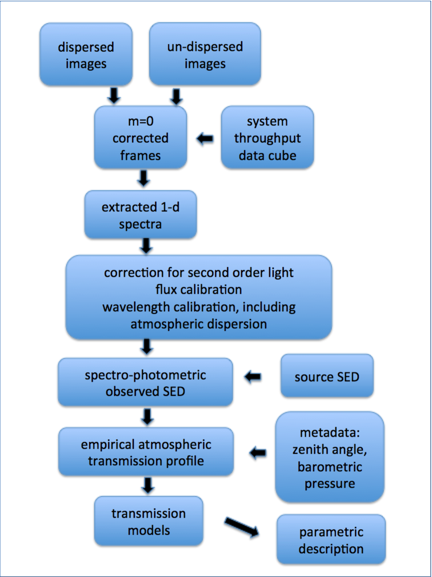
\includegraphics[width=\textwidth]{figures/aux_telescope_workflow.png}
	\caption{Flowchart depicting the atmospheric absorption measurement pipeline.}.
	\label{fig:aux_telescope}
\end{figure}

The 1D spectra are then extracted from the image, flux calibrated, and corrected for second order light contamination\footnote{ It should be noted that strictly speaking, second order light contamination invalidates the flat-fielding method described above. If the effect is small, a simple QE curve will likely suffice to correct for this effect, otherwise an iterative approach to the flat-fielding will be taken.}. A more precise wavelength calibration is then performed using the spectral lines in this corrected spectrum, taking into account the effect of differential chromatic refraction, resulting in a spectrophotometrically calibrated measurement.

The \hyperref[sec:CPP:output:spectrophotometricStandards]{source's true SED} and the calibrated spectrophotometric observation are then used in conjunction with the observational meta-data, \eg the zenith angle, temperature, and barometric pressure, to derive an empirical measurement of the atmospheric transmission. This absorption profile is then fitted to an atmospheric transmission model to improve the delivered spectral absorption measurement, as well to provide a parametric description of the state of the atmosphere at the time of observation.


 
\subsubsection{Night Sky Spectrum}\label{sec:CPP:aux:nightSkySpectrum}
The acquisition of a night sky spectrograph is unlikely as it is not in the baseline design specification. However, in the eventuality that such an instrument is obtained, we provision for the determination of the emission spectrum of the night sky near the \auxtelescope boresight, with $R \sim 200$\footnote{ It is not entirely clear yet whether these will be taken on the Calypso or the 8.4m boresight.}, which will be used to synthesize flat-field images matching the sky's SED using the \hyperref[sec:CPP:output:monoFlat]{monochromatic dome flats}.
\alg Assuming we have a sky spectrograph this is simple. In the absence of a sky spectrograph, an $R \sim 10$ spectrum will be acquired using standard/narrowband filters. Furthermore, if the fringe structures are sufficiently stable, \ie they are well described by \smalltilde 3 PCA components, we may be able to simply use a classic fringe subtraction.



%%%%%%%%%%%%%%%%%%%%%%%%%%%%%%%%%%%%%%%%%%%%%%%%%%%%%
%%%%%%%%%%%%%%%%%%%%%%%%%%%%%%%%%%%%%%%%%%%%%%%%%%%%%
%%%%%%%%%%%%%%%%%%%%%%%%%%%%%%%%%%%%%%%%%%%%%%%%%%%%%

% The following is commented out as it's not a DM deliverable, but lives on here just in case...
%\subsection{Miscellaneous Algorithms}\label{sec:CPP:miscAlg}
%\begin{itemize}
%	\item Ghosting model: Following the above analysis we will have information which, whilst not needed to perform the calibration of LSST, will provide a valuable cross-check, and will inform the camera and telescope teams about the state of the optical elements, and is therefore an output of the Calibration Products Pipeline. This can be done in two ways:
%	\mysubitem By analysis of the CBP data, concentrating not on the spots but on the scattered/ghost light.
%	\mysubitem By looking at the corrections applied to the CBP spot data to arrive at the dome screen data.
%\end{itemize}





%%%%%%%%%%%%%%%%%%%%%%%%%%%%%%%%%%%%%%%%%%%%%%%%%%%%%
%%%%%%%%%%%%%%%%%%%%%%%%%%%%%%%%%%%%%%%%%%%%%%%%%%%%%
%%%%%%%%%%%%%%%%%%%%%%%%%%%%%%%%%%%%%%%%%%%%%%%%%%%%%





\subsection{Photometric calibration walk-through}
\label{sec:CPP:walkthrough}
The Calibration Products Production section aims to provide all the ingredients necessary to photometrically calibrate the entire LSST survey, visit-by-visit and band-to-band, thus arriving at everything except a single photometric zero-point for the survey.

The effective end-to-end instrumental throughput, as a function of wavelength, focal-plane/pupil position, and time, is known from the \hyperref[sec:CPP:output:monoPhotoFlat]{ghost-corrected monochromatic flat-fields} and the \hyperref[sec:CPP:output:filterTransmission]{filter transmission functions}.

The atmospheric transmission as a function of wavelength, at the time each observation is made, is known at some position in the field-of-view by taking the ratio of \hyperref[sec:CPP:output:spectrophotometricStandards]{spectrophotometricly calibrated stellar spectrum} of a bright ($8^{\text{th}}-10^{\text{th}}$ magnitude) star, as measured by the \auxtelescope, to the BP/RP spectrum as measured above the atmosphere by Gaia. 


It should be noted that the effective delivered spectral resolution of both the \hyperref[sec:CPP:output:spectrophotometricStandards]{Gaia spectrophotometry} and the \hyperref[sec:CPP:aux:atmosphericAbsorption]{atmospheric absorption} can be improved using model fits. The stellar spectra from Gaia, with ($R \sim 40-70$) for the BP and RP spectra respectively\cite{GaiaSpecs}, can be fitted to standard stellar spectral types, as will be done internally by Gaia for their data releases\cite{BailerJones10}. For the atmospheric absorption profile, as described in \secsymbol\ref{sec:CPP:aux:atmosphericAbsorption}, the absorption features from the atmosphere will be fitted to an atmospheric transmission model (\eg MODTRAN \etc), allowing us to improve the delivered measurement of the spectral absorption features present at the time of observation. 
%How necessary it will be to enhance the stellar spectra provided by Gaia depends both on Gaia's delivered performance at GRDR3, and on the delivered performance of the \auxtelescope, as we need to match its performance at a minimum.
%% Above line is commented out, as I think we plan to use the stellar model fitting from Gaia whatever happens.


Images are flat-fielded using the color of the sky at the time of observation, and then re-flatfield with some pre-selected SED\footnote{ Whether this is a flat SED, some nominal SED \eg a G-star's, remains TBD.}. After this, per-object corrections are made, to correct for both the object's assumed SED and the atmospheric transmission at the time of observation. 
%With each object correctly flat-fielded, and the atmospheric transmission and system response function corrected for in each visit, the entire visit has a photometric zeropoint assigned by fitting the stars in the visit to those in the \hyperref[sec:CPP:output:spectrophotometricStandards]{spectrophotometric catalogue.}, leaving each visit in each band corrected and tied together.
With each object now flat-fielded with the appropriate spectrum, and the atmospheric transmission and system response functions corrected for in each visit, the photometric zero-point for the visit is fitted using the \hyperref[sec:CPP:output:spectrophotometricStandards]{photometric standard star set}. This therefore leaves just the overall flux level unknown, thus bringing us to one global photometric zero-point for the entire survey.


This whole-survey zero-point can then calculated using an empirical approach to tie this back to the definition of the Jansky, and two proposals exist for doing so. The first is to use CBP measurements in conjunction with NIST calibrated photodiodes in the CBP's integrating sphere to measure the absolute instrumental sensitivity, though this will require integrating over the pupil. The second is to use a `son-of-StarDICE' type approach, where precisely calibrated and stabilized LEDs of known wavelength and luminosity are observed by either LSST (or the \auxtelescope, as their observations are already tied together), allowing the absolute system response to be measured using observations which illuminate the entire pupil at a set of wavelengths.
















It should be noted that it is not yet known whether the atmospheric transmission will vary significantly across LSST's field of view, and that this is currently being measured for the first time by wide-field cameras such as DECam and HSC. Should it turn out that the atmospheric transmission varies on spatio-temporal scales relevant to the survey, we propose to make further per-visit corrections by measuring the variation in flux as a function of color/spectral classification for all Gaia sources across the field of view. However, should this not be necessary, measuring this variation anyway will allow the spatial structure of the atmospheric transmission to be constrained, providing a convenient quality-assurance null-test to validate this choice.





%\hyperref[sectionlink]{text} 
%\hyperref[sectionlink]{text} 
%\hyperref[sectionlink]{text} 
%\hyperref[sectionlink]{text} 
%\hyperref[sectionlink]{text} 
%\hyperref[sectionlink]{text} 



%%%%%%%%%%%%%%%%%%%%%%%%%%%%%%%%%%%%%%%%%%%%%%%%%%%%%
%%%%%%%%%%%%%%%%%%%%%%%%%%%%%%%%%%%%%%%%%%%%%%%%%%%%%
%%%%%%%%%%%%%%%%%%%%%%%%%%%%%%%%%%%%%%%%%%%%%%%%%%%%%

\subsection{Prototype Implementation}
\label{sec:CPP:prototypeImplementation}
While parts of the Calibration Products Pipeline have been prototyped by the LSST Calibration Group (see the \NewPCP for discussion), these have not been written using LSST Data Management software framework or coding standards. We therefore expect to transfer the know-how, and rewrite the implementation.











%%%%%%%%%%%%%%%%%%%%%%%%%%%%%%%%%%%%%%%%%%%%%%%%%%%%%
%%%%%%%%%%%%%%%%%%%%%%%%%%%%%%%%%%%%%%%%%%%%%%%%%%%%%
%%%%%%%%%%%%%%%%%%%%%%%%%%%%%%%%%%%%%%%%%%%%%%%%%%%%%

%This WBS is responsible for the development of the data analysis algorithms and software required and the ultimate delivery of the flat fields. Development and commissioning of the CBP itself, together with any other infrastructure required to perform the above procedure, lies outwith Data Management (see 04C.08 \emph{Calibration System}).
%
%\paragraph{Atmospheric transmissivity}
%
%Measurements from the auxiliary instrumentation---to include the 1.2\,m ``Calypso'' telescope, a bore-sight mounted radiometer and satellite-based measurement of atmospheric parameters such as pressure and ozone---will be used to determine the atmospheric absorption along the line of sight to standard stars. The atmospheric transmission will be decomposed into a set of basis functions and interpolated in space in time to any position in the LSST focal plane.
%
%This WBS will develop a pipeline for accurate spectrophotometric measurement of stars with the auxiliary telescope. We expect to repurpose and build upon publicly available code e.g.\ from the PFS\footnote{Subaru's Prime Focus Spectrograph; \url{http://sumire.ipmu.jp/pfs/}.} project for this purpose.
%
%This WBS will construct the atmospheric model, which may be based either on \textsc{modtran} (as per \NewPCP{}) or a PCA-like decomposition of the data (suggested by \cite{Lupton15}).
%
%This WBS will define and develop the routine for fitting the atmospheric model to each exposure from the calibration telescope and providing estimates of the atmospheric transmission at any point in the focal plane upon request.
%
%\paragraph{Detector effects}
%
%An initial cross-talk correction matrix will be determined by laboratory measurements on the Camera Calibration Optical Bench (CCOB). However, to account for possibile instabilities, this WBS will develop an on-telescope method. We baseline this as being based on measurement with the CBP, but we note the alternative approach based on cosmic rays adopted by HSC \cite{Furusawa14}.
%
%Multiple reflections between the layers of the CCD give rise to spatial variability with fine scale structure in images which may vary with time \cite[\S2.5.1]{Lupton15}. These can be characterized by white light flat-fields. Preliminary analysis indicates that these effects may be insignificant in LSST \cite{Rasmussen15}; however, the baseline calls for a routine developed in this WBS to analyse the flat field data and generate fringe frames on demand. This requirement may be relaxed if further analysis (outside the scope of this WBS) demonstrates it to be unnecessary.
%
%
%This WBS will develop algorithms to characterize and mitigate anomalies due to the nature of the camera's CCDs.
%
%\begin{note}
%There's a complex inter-WBS situation here: the actual mitigation of CCD anomalies will generally be performed in SFM (\wbsSFM{}), based on products provided by this WBS which, in turn, may rely on laboratory based research which is broadly outside the scope of DM\@. We baseline the work required to develop the corrective algorithms here. We consider moving it to \wbsSFM{} in future.
%\end{note}
%
%The effects we anticipate include:
%
%\begin{itemize}
% \item{QE variation between pixels;}
% \item{Static non-uniform pixel sizes (e.g.\ ``tree rings'' \cite{Stubbs14});}
% \item{Dynamic electric fields (e.g.\ ``brighter-fatter'' \cite{Antilogus14});}
% \item{Time dependent effects in the camera (e.g.\ hot pixels, changing cross-talk coefficients);}
% \item{Charge transfer (in)efficiency (CTE).}
%\end{itemize}
%
%Laboratory work required to understand these effects is outwith the scope of this WBS\@. In some cases, this work may establish that the impact of the effect may be neglected in LSST\@. The baseline plan addresses these issues through the following steps:
%
%\begin{itemize}
% \item{Separate QE from pixel size variations\footnote{Refer to work by Rudman.} and model both as a function of position (and possibly time);}
% \item{Learn how to account for pixel size variation over the scale of objects (e.g.\ by redistributing charge);}
% \item{Develop a correction for the brighter-fatter effect and develop models for any features which cannot be removed;}
% \item{Handle edge/bloom using masking or charge redistribution;}
% \item{Track defects (hot pixels);}
% \item{Handle CTE, including when interpolating over bleed trails.}
%\end{itemize}
%


%

%Produce Master Pupil Ghost Exposure; Determine CCOB-derived Illumination Correction; Determine Optical Model-derived Illumination Correction; Determine Star Raster Photometry-derived Illumination Correction; Create Master Illumination Correction; Determine Self-calibration Correction-Derived Illumination Correction; Correct Monochromatic Flats; Reduce Spectrum Exposure


%%%%%%%%%%%%%%%%%%%%%%%%%%%%%%%%%%%%%%%%%%%%%%%%%%%%%
%%%%%%%%%%%%%%%%%%%%%%%%%%%%%%%%%%%%%%%%%%%%%%%%%%%%%
%%%%%%%%%%%%%%%%%%%%%%%%%%%%%%%%%%%%%%%%%%%%%%%%%%%%%

%\subsection{UNSTRUCTURED OPEN QUESTIONS \\ a.k.a. Merlin's random thoughts/ramblings}\label{sec:calibQuestions}

%This section is just things that I thought of whilst working through this document. They probably don't belong in here at all, but I wanted to capture them and this seemed a semi-relevant place (and Jim started it!).
%\begin{itemize}
%	\item Flat fielding the auxiliary telescope: What is required? What are the plans? We have a flat-field screen in this dome, correct? (Now confirmed) Regarding the bandpasses, what do we have in terms of filters? (Answer: full LSST set on the imager) What do we need? Is it not necessary get an accurate throughput determination at 1nm resolution by taking the CBP or at least the monochromatic laser source over there for a one-off characterization? (Answer: the laser is not going to happen but there is a monochromatic light source in the \auxtelescope\ baseline.) If not, how are we accurately characterizing the response of the detector which will itself be doing the $R \sim 200$ spectrophotometry of the standard stars?
%	\begin{note}
%		Need to go back and add in doing monochromatic composite flat-fielding of this telescope, \emph{and} add that these need to be applied somewhere/somehow. The application of \emph{these} to the \auxtelescope\ data really doesn't belong in AP or DRP as all the other photocal stuff does.
%	\end{note}
	
%	\item Crosstalk coupling: depending on where this happens in the electronic chain, this may be ``conservative" or ``generative", \ie\ if the crosstalk is from a capacitive coupling at an early stage of the readout then the crosstalk which is removed from the victims should be added back in to the aggressors, as this is signal which has been \emph{lost}. However, if it occurs after a significant amount of amplification (likely), then it should just be removed. Again, I'm sure this is known but I'd just like to check as this matters at the sub 1\% level. \rednote{Answer: Very likely generative, but the reasoning for this assumes a low impedance on the output analog lines (such that the voltage does not drop when capacitive coupling occurs) but this is actually not necessarily the case, and perhaps should be checked more thoroughly. Can likely persuade Paul O'Connor/Andrei Nomerotski/Hyeyun Park to investigate if necessary.}
	
%	\item Crosstalk (again): I am lead to believe that crosstalk correction will be applied in the DAQ. If this is correct, then this point is just to note that the calibration system needs to be able to disable this and access the truly raw images in order to make the crosstalk matrix measurements using CBP spots. It will also need to be able to push a new crosstalk matix to the DAQ to confirm meaurements (and to update the system in general). \rednote{RHL says this is already captured somewhere relevant.}
	
%	\item Crosstalk (yet again): Has anyone considered the nightmare scenario where crosstalk is a function of alt, az and rotator position due to changes in these couplings from cable movement? Or is this certain to be only a 1\% change in a 1\% effect, and therefore not a concern? \rednote{Answer: Turns out that it really is very unlikely indeed, as almost everything comes from intra-flex-cable coupling and wire-bond coupling, which won't move when the camera is repositioned.}
	
%	\begin{note}
%		Need to include algorithm for applying crosstalk corrections after the fact in the event that the data-buffer overflows in the case of internet outages between the summit and the US. The also implies that a time history of the measured crosstalk matrices needs to be stored somewhere.
%	\end{note}
		
%	\item Does bleeding occur only in the serial register? (surely not) If not then why do we expect it to be a per-amplifier thing particularly, rather than a per pixel effect, as it is presumably defined by the depth of each well? This is surely known, but I should discuss with someone. \rednote{Answer: There is more than one thing here: bleeding/blooming $\neq$ saturation. Blooming levels are a per-pixel effect (though likely very similar throughout a chip), whilst ``saturation'' is in the amplifier/ADC, which is obviously per-channel. }
	
%	\item Pulse-to-pulse variation in the narrowband laser. When averaged over, what is the RMS? And how stable is the mean over time? (I have met lasers which drift \bfeffect{like crazy}). How do these properties change as one sweeps the wavelength around as would be required for taking the 20nm width flats?
	

%\end{itemize}






\clearpage































%%%%%%%%%%%%%%%%%%%%%%%%%%%%%%%%%%%%%%%%%%%%%%%%%%%
%%%%%%%%%%%%%%%%%%%%%%%%%%%%%%%%%%%%%%%%%%%%%%%%%%%
%%%%%%%%%%%%%%%%%%%%%%%%%%%%%%%%%%%%%%%%%%%%%%%%%%%



%\section{Photometric Calibration Pipeline (\wbsPhotoCal)}
%
%\subsection{Key Requirements}
%
%The Photometric Calibration Pipeline is required to internally calibrate the relative photometric zero-points of every observation, enabling the Level 2 catalogs to reach the required SRD precision.
%
%\subsection{Baseline Design}
%
%The adopted baseline algorithm is a variant of ``ubercal'' \cite{Padmanabhan08, Schlafly12}. This baseline is described in detail in the Photometric Self Calibration Design and Prototype Document (\UCAL).
%
%\subsection{Constituent Use Cases and Diagrams}
%
%Perform Global Photometric Calibration;
%
%\subsection{Prototype Implementation}
%
%Photometric Calibration Pipeline has been fully prototyped by the LSST Calibration Group to the required level of accuracy and performance (see the \UCAL document for discussion). % RHL really? I thought that they wrote a small-scale toy version. But I may be totally out of date.
%\\
%
%As the prototype has not been written using LSST Data Management software framework or coding standards, we assume a non-negligible refactoring and coding effort will be needed to convert it to production code in LSST Construction.
%
%\clearpage
%
%\section{Astrometric Calibration Pipeline (\wbsAstroCal)}
%
%\subsection{Key Requirements}
%
%The Astrometric Calibration Pipeline is required to calibrate the relative and absolute astrometry of the LSST survey, enabling the Level 2 catalogs to reach the required SRD precision.
%
%\subsection{Baseline Design}
%
%Algorithms developed for the Photometric Calibration Pipeline (\wbsPhotoCal) will be repurposed for astrometric calibration by changing the relevant functions to minimize. This pipeline will further be aided by WCS and local astrometric registration modules developed as a component of the Single Frame Processing pipeline (\wbsSFM).
%\\
%
%Gaia standard stars will be used to fix the global astrometric system. It is likely that the existence of Gaia catalogs may make a separate Astrometric Calibration Pipeline unnecessary.
%
%\subsection{Constituent Use Cases and Diagrams}
%
%Perform Global Astrometric Calibration;
%
%\subsection{Prototype Implementation}
%
%The Astrometric Calibration Pipeline has been partially prototyped by the LSST Calibration Group, but outside of LSST Data Management software framework. We expect to transfer the know-how, and rewrite the implementation.
